% Conference version for the 2027 IEEE 7th International Conference on Smart
% Information Systems and Technologies (SIST), Astana, 12-14 May 2027.
% Requirements: IEEE two-column conference format, A4, 4-6 pages, English, PDF.
% Every number was checked against the generated tables in
% ml/experiments/inflation/results/tables/ (see README.md in this folder).
% Build: see README.md in this folder.
\documentclass[conference,a4paper]{IEEEtran}
\IEEEoverridecommandlockouts
\usepackage{cite}
\usepackage{amsmath}
% Times is required by the template. pdfLaTeX gets it from IEEEtran itself;
% XeLaTeX/LuaLaTeX and Tectonic need the OpenType clone TeX Gyre Termes.
\usepackage{iftex}
\ifPDFTeX\else
  \usepackage{fontspec}
  \usepackage{unicode-math}
  \setmainfont{texgyretermes}[Extension=.otf, UprightFont=*-regular,
    BoldFont=*-bold, ItalicFont=*-italic, BoldItalicFont=*-bolditalic,
    Ligatures=TeX]
  \setmathfont{texgyretermes-math.otf}
\fi
\usepackage{graphicx}
\usepackage{booktabs}
\usepackage{array}
\usepackage{flushend}
\usepackage[hidelinks]{hyperref}
\hypersetup{pdftitle={Feature Injection Can Inflate the Performance of Quiz-Cheating Detectors: Evidence From Behavior-Level Simulation},
  pdfauthor={Aitbek Kaiyrbekuly, Aivar Sakhipov}}
\renewcommand{\IEEEkeywordsname}{Keywords}
\newcommand{\pp}{\,pp}

\begin{document}
\bstctlcite{IEEEexample:BSTcontrol}

\title{Feature Injection Can Inflate the Performance of Quiz-Cheating Detectors: Evidence From Behavior-Level Simulation}

% Two authors, as decided on 15 Nov 2026. The public repository does not hold
% e-mail addresses: `submission.tex` builds the version for upload with the
% author block from `authors.local.tex` (git-ignored; copy authors.example.tex).
\ifdefined\AuthorBlockFile
  \input{\AuthorBlockFile}
\else
\author{\IEEEauthorblockN{Aitbek Kaiyrbekuly}
\IEEEauthorblockA{\textit{School of Software Engineering} \\
\textit{Astana IT University}\\
Astana, Kazakhstan \\
e-mail to be added}
\and
\IEEEauthorblockN{Aivar Sakhipov}
\IEEEauthorblockA{\textit{School of Software Engineering} \\
\textit{Astana IT University}\\
Astana, Kazakhstan \\
e-mail to be added}
}
\fi

\maketitle

\begin{abstract}
Detectors of cheating in online quizzes are rarely evaluated on verified cases. Positive cases are instead simulated, injected or labeled by heuristics, and the evaluation becomes circular when their definition shares features with the detector. We study the most direct such construction, feature-aligned injection, in a paired simulation. Three detectors frozen in advance (quantile rules, and an Isolation Forest with and without peer features) are evaluated twice on the same simulated students: once with anomalies injected along the detectors' own features, and once with cheating simulated as behavior (pre-knowledge, answer look-up, peer copying and proxy test-taking) on top of an item-response and response-time model calibrated on the EdNet data set. With the original injection recipes, recall at a 5\% false-positive rate falls from 46--62\% to 23--36\%, and a gradient-boosting classifier trained on injected labels loses 35 percentage points. The gap is not a constant. It is largest for look-up and for peer copying seen through peer features, whose synchrony condition the collusion recipe always satisfies; it is absent or slightly negative for proxy test-taking and changes sign when the injected dose is lowered. Recall measured on feature-aligned injection therefore does not predict recall on behavior-level cheating. On real EdNet logs, detectors without peer features that were fitted on synthetic ordinary behavior flag two to eight times the nominal 5\% of attempts. We give recommendations for evaluating log-based cheating detectors.
\end{abstract}

\begin{IEEEkeywords}
academic integrity, online assessment, anomaly detection, cheating detection, synthetic data, evaluation methodology, learning analytics
\end{IEEEkeywords}

\section{Introduction}
Online quizzes leave a detailed trace of how a student worked: when each question was shown, how long the first answer took, whether it was later changed, and when the attempt was submitted. A substantial share of students report having cheated in online exams \cite{newton2024howcommon}, and a growing body of work mines these traces with statistical rules, anomaly detectors or classifiers \cite{noorbehbahani2022review}. Such detectors are attractive for learning management systems (LMS) because they need no camera and no data beyond what the platform already logs.

The weak point of this line of work is evaluation. Verified cases of cheating are rare, confidential, and biased toward what existing procedures already catch. We coded a scoping sample of 48 studies from 2015--2026 by the provenance of their positive cases (non-systematic search with snowballing, one coder; search description and list are published with our code). Six studies evaluated on cheating induced experimentally in real participants and six on cases confirmed or flagged independently of the detector (five of these on one credentialing data set). The others had no labeled positives (9), labeled real data with a heuristic or another detector (12), simulated cheating with a psychometric model (12), or altered records by a rule (3).

Several of these constructions share one risk. When positive cases are defined through quantities that the detector itself measures, or are generated by the model family on which the detector is built, the evaluation partly measures the agreement between the construction and the detector. In test security, Belov and Toton call validation on simulated aberrance biased for this reason \cite{belov2022realdata}, and Gorney and Wollack show that the generating model changes the measured power of pre-knowledge detectors \cite{gorney2022generating}.
For log-based detectors in learning platforms this effect has not been examined under controlled conditions. We examine it for the construction in which the circularity is most direct, and which the platform that motivated this study used itself: \emph{feature-aligned injection}. Ordinary attempts are perturbed along the detector's features, so that answers become faster, are changed more often, two students receive the same answers at the same moment, or the score jumps. Real misconduct is a behavior with a mechanism, and its footprint in the log is a by-product of that mechanism. It may be weak, spread over several features, or opposite in sign to the injected one: looking an answer up makes a student slower, not faster.

We evaluate three detectors that were frozen before the experiment on \emph{paired counterfactual worlds}: the same simulated students, honest attempts and cheaters are rendered once with feature-aligned injection and once with cheating simulated as behavior. The pairing removes differences in the population. It does not remove the choice of how strongly students cheat, so we vary the dose of both constructions. The contributions are (i) an open behavior-level simulator of quiz attempts with four cheating mechanisms, calibrated on public data and emitting events in the contract of the Examory learning platform under development at our university; (ii) the paired comparison with dose, sensitivity and protocol analyses for unsupervised detectors, a supervised classifier and two classical indices; and (iii) false-positive estimates on real logs. The detectors produce risk signals for review by a teacher; none of the results shows that statistical flags can establish misconduct.

\section{Related Work}
\textbf{Evaluation data in cheating detection.} In the machine-learning part of our sample (23 studies), nine have no labeled positives, as in work on multiple-account cheating \cite{northcutt2016cameo}; ten label real data with a heuristic rule or with the output of another detector \cite{ruiperez2019multiple,alexandron2024general}; and two inject synthetic cases \cite{kamalov2021cheating,shatnawi2025moodle}. In the psychometric part (25 studies), twelve simulate cheating with a psychometric model, in at least four cases of the detector's own family, and one shifts real response times on compromised items for a statistic that tests for faster times on those items \cite{sinharay2020rt}. Among the 15 studies with injected or heuristically labeled positives, the definition of a positive overlaps with the detector's inputs in five and partly in four. Some authors avoid the overlap deliberately, for example by removing from the inputs the times that defined the label \cite{erdem2025cheating}. Strict feature-aligned injection is thus uncommon in this sample; constructions that share assumptions with the detector are not.

\textbf{Psychometric indices and field experiments.} Educational measurement offers indices for specific forms of fraud, whose power depends on how much of the test is affected and on how the fraud is carried out \cite{cizek2017handbook}. Two field experiments are the closest external anchors. Ranger \emph{et al.} induced several forms of cheating in a 20-item mock exam and compared old and new indicators \cite{ranger2020eexams}; we use their detection rates and revision counts in Section~\ref{sec:discussion}. Toton and Maynes disclosed 12 of 25 items to randomly assigned examinees \cite{toton2019preknowledge}.

\textbf{Synthetic evaluation in other fields.} The construction of anomalies drives benchmark conclusions in outlier detection \cite{emmott2013benchmarks}. Intrusion detection met the same criticism of unvalidated synthetic backgrounds that do not transfer to operation \cite{mchugh2000testing,sommer2010outside}, as did time-series benchmarks \cite{wu2023benchmarks}, security research \cite{arp2022dos} and work on data leakage \cite{kapoor2023leakage}. Simulated learners often lack evidence of validity \cite{kaser2024simulated}, and guidance on simulation studies asks for explicit data-generating mechanisms, estimands and Monte Carlo errors \cite{morris2019simulation}.

\section{Methods}
\subsection{Design}
The experiment holds the detectors fixed and varies the evaluation data. In condition SIM-FI, ordinary behavior comes from a latent learner model calibrated on real logs and cheating attempts are produced by feature-aligned injection. In SIM-BL, the same students, items, honest attempts, cohorts and cheaters are used, and cheating attempts are produced by behavior-level mechanisms. Each cheater has one type, and each type has an injected and a behavioral form (Table~\ref{tab:types}). The quantity of interest is the difference in a detector's recall between the two worlds at the same false-positive rate (FPR). A third condition, LEGACY, is the platform's original generator: ad hoc ordinary behavior, the same recipes and constants, and its own random draws.

All conditions share one assessment format: cohorts of 20 students, a 20-item four-option quiz, three attempts per student on the same form, and cheating only on the final attempt. In the main experiment 12\% of all attempts (36\% of final attempts) are cheating attempts, with the shares of Table~\ref{tab:types}; a separate analysis uses 5\% of final attempts. Each replicate has 2,000 students, and 20 replicates are generated per condition unless stated otherwise.

\begin{table}[t]
\caption{Cheating Types, Their Share of Cheating Attempts, and Their Injected and Behavioral Forms}
\label{tab:types}
\centering
\footnotesize
\setlength{\tabcolsep}{3pt}
\renewcommand{\arraystretch}{1.05}
\begin{tabular}{@{}>{\raggedright\arraybackslash}p{0.15\columnwidth}>{\raggedright\arraybackslash}p{0.37\columnwidth}>{\raggedright\arraybackslash}p{0.42\columnwidth}@{}}
\toprule
Type & Injection (SIM-FI) & Behavior (SIM-BL) \\
\midrule
Pre-know\-ledge, 35\% & \emph{Rapid response}: each answer time, w.p.\ 0.65, $\times$0.18--0.55 & Item leaked w.p.\ 0.65, recalled w.p.\ 0.92; half answer fast, half disguise timing \\
Look-up, 25\% & \emph{Excessive changes}: each item, w.p.\ 0.45--0.75, gets 1--4 changes & Unknown item looked up w.p.\ 0.70 (${\approx}35$\,s, success 0.90); half answer first, correct later \\
Peer copying, 25\% & \emph{Collusion}: shared answers, 30\% of items one wrong option, submission within 1\,s & Copier follows a source (the abler student w.p.\ 0.80), copies each item w.p.\ 0.80; half of the pairs submit together \\
Proxy, 15\% & \emph{Score jump}: $P(\text{correct})$ $+$0.18--0.32 & Abler person takes the final attempt \\
\bottomrule
\multicolumn{3}{@{}l}{w.p.: with probability.}
\end{tabular}
\end{table}

\subsection{Detectors and Protocol}
The detectors are those of the Examory LMS as tagged before the simulator existed; their code was not modified. Each attempt is described by twelve attempt-level features (first-answer time summaries, the fraction of unusually fast answers, duration, answer changes, the score, and its standardized difference from the student's earlier attempts) and three peer features computed against students of the same cohort who submitted within $\pm 5$\,s: their number and two measures of answer agreement. \emph{Rules} scores an attempt by its most extreme two-sided rank relative to ordinary training attempts over all fifteen features, the peer features included. \emph{IF} is an Isolation Forest \cite{liu2008isolation} on the twelve attempt-level features only, and \emph{IF+peers} is the same forest on all fifteen. Rules and IF+peers are therefore the two detectors with peer features.

Cohorts are split 60/20/20 into training, validation and test sets. Models are fitted on ordinary training attempts, the threshold is the point of maximum validation recall subject to an FPR of at most 5\%, and all metrics are computed on test cohorts. The protocol contains two oracles that later analyses remove: the threshold uses validation labels, and the training data are purged of cheating attempts.

\subsection{Feature-Aligned Injection}
The four recipes of the platform's generator (Table~\ref{tab:types}, middle column) are applied to the final attempts of the cheaters, each along one family of features: answer times, answer changes, peer agreement and synchrony, and score. An injection dose $\lambda$ multiplies the per-item probabilities, the copy probability and the score shift; $\lambda = 1$ is the original recipe. The forced-wrong items and the synchronous submission are not scaled.

\subsection{Behavior-Level Simulation}
\textbf{Honest behavior.} A student has an ability, a speed, a disengagement propensity and a revision propensity. Correctness follows the three-parameter logistic model and response times a lognormal model \cite{vanderlinden2006lognormal,vanderlinden2007hierarchical}; disengaged responses are rapid guesses \cite{wise2005rte}; answers may be revised. All parameters are estimated with our own code (joint maximum a posteriori for the item-response model, 1,089 items) from EdNet-KT2 \cite{choi2020ednet}, the action log of a language-tutoring service, on one half of the users, a fifth of whom are held out to check the fit. On the held-out users the fitted model reproduces first-answer times well but produces fewer answer changes than real attempts (4.5 against 6.7 per attempt).

\textbf{Cheating mechanisms.} Cheating is simulated as actions on top of the honest attempt of the same student, re-using the student's random draws (Table~\ref{tab:types}, right column). An intensity $x$ replaces the per-item coverage of the first three mechanisms and scales the ability gain of the proxy. These parameters are assumptions; the sensitivity analysis varies them, including the shares of cheaters who disguise their timing, answer before correcting, or submit together, each over 0--1. Attempts not touched by cheating are byte-identical across worlds.

\subsection{Real Data}
The other half of EdNet-KT2 is cut into attempts of 20 consecutive responses and converted into the same event format, which yields 23,042 attempts of 10,671 users. The service is an ungraded self-study tutor, so we read the share of flagged attempts as an FPR. Detectors are either fitted on synthetic ordinary attempts and applied unchanged, or refitted on real attempts. Realism is quantified by a classifier two-sample test \cite{lopezpaz2017c2st}.

\subsection{Analyses and Statistics}
The primary outcome, fixed before the multi-replicate runs, is the paired difference in recall between SIM-FI and SIM-BL per detector and type, with Holm correction over the twelve tests \cite{holm1979simple}. The plan was not preregistered, and the reported run with calibrated parameters followed a first full run with uncalibrated defaults under the same outcome, correction and decision rules; that run is published with the code. The following analyses were added after the main results had been seen and are exploratory: recall by sub-population; the dose grid; a sensitivity analysis over 14 parameters (60 Latin-hypercube configurations, 10 replicates each); protocol and honest-behavior variants; a supervised classifier; and an answer-similarity and a response-time person-fit index \cite{marianti2014aberrant}. Values are means over replicates with bootstrap 95\% intervals, which quantify Monte Carlo error under fixed code and parameters (Monte Carlo standard errors at most 3\pp{}). Because $p$-values in a simulation shrink with the number of replicates, the intervals are the main summary. Differences are tested with an exact sign-flip permutation test, which replaced the Wilcoxon signed-rank test of the original plan; Table~\ref{tab:main} marks the one result that depends on this choice. Percentage points are abbreviated pp.

\section{Results}
\subsection{Performance at the Default Constants}
The realized FPR is 4.2--5.3\% in every condition. Table~\ref{tab:main} gives recall. Each detector loses 23--26\pp{} of overall recall when injection is replaced by behavior-level cheating, but the picture per type is uneven. All detectors lose 54--70\pp{} on look-up. The two detectors with peer features lose 35 and 39\pp{} on peer copying, while IF detects behavior-level copying better than injected collusion. The forests lose 11 and 26\pp{} on pre-knowledge and the rules nothing. No detector reaches 15\% recall on proxy test-taking in either world. The ordinary behavior into which anomalies are injected matters as well: on the original generator (LEGACY) the rules detect pre-knowledge 15.4\pp{} better than under behavior-level cheating.

\begin{table}[t]
\caption{Recall (\%) at the 5\% FPR Threshold and Paired Difference Between the Injected and Behavioral Worlds (20 Replicates)}
\label{tab:main}
\centering
\footnotesize
\setlength{\tabcolsep}{3pt}
\begin{tabular}{@{}llrrrr@{}}
\toprule
Detector & Type & LEGACY & SIM-FI & SIM-BL & Diff. [95\% CI] \\
\midrule
Rules & all & 68.6 & 61.9 & 36.2 & 25.8 [23.0, 28.6] \\
 & pre-kn. & 49.7 & 34.1 & 34.3 & $-$0.2 [$-$6.1, 5.3] \\
 & look-up & 99.0 & 97.8 & 28.0 & 69.8 [64.9, 74.6]$^{*}$ \\
 & copying & 100.0 & 100.0 & 65.5 & 34.5 [29.1, 39.9]$^{*}$ \\
 & proxy & 14.0 & 12.3 & 10.7 & 1.6 [$-$3.3, 6.9] \\
\midrule
IF & all & 40.6 & 46.3 & 22.9 & 23.4 [21.0, 25.8] \\
 & pre-kn. & 57.9 & 55.6 & 29.8 & 25.7 [23.0, 28.4]$^{*}$ \\
 & look-up & 74.1 & 91.1 & 23.2 & 67.9 [64.7, 71.0]$^{*}$ \\
 & copying & 1.4 & 11.0 & 21.5 & $-$10.5 [$-$14.3, $-$6.7]$^{*}$ \\
 & proxy & 6.3 & 5.6 & 8.3 & $-$2.7 [$-$5.5, 0.1] \\
\midrule
IF+peers & all & 48.6 & 53.6 & 27.8 & 25.8 [23.9, 27.7] \\
 & pre-kn. & 38.6 & 35.4 & 24.2 & 11.2 [8.0, 14.7]$^{*}$ \\
 & look-up & 50.0 & 68.0 & 14.4 & 53.6 [48.8, 58.3]$^{*}$ \\
 & copying & 88.8 & 100.0 & 61.0 & 39.0 [34.6, 43.5]$^{*}$ \\
 & proxy & 6.6 & 5.1 & 9.5 & $-$4.4 [$-$6.6, $-$2.2]$^{\dagger}$ \\
\bottomrule
\multicolumn{6}{@{}l}{Diff.: SIM-FI $-$ SIM-BL. LEGACY (original generator) is not paired.} \\
\multicolumn{6}{@{}l}{$^{*}$Holm-adjusted $p < 0.01$ (12 tests; sign-flip and Wilcoxon).} \\
\multicolumn{6}{@{}l}{$^{\dagger}$Holm-adjusted $p = 0.007$ (sign-flip), $0.016$ (Wilcoxon).}
\end{tabular}
\end{table}

\subsection{Dependence on the Dose of Both Constructions}
Table~\ref{tab:main} holds for one injected dose and one behavioral intensity. Fig.~\ref{fig:dose} crosses four doses with five intensities (10 replicates, so its values differ slightly from Table~\ref{tab:main}). For pre-knowledge and look-up the difference changes sign inside the grid. At the default intensity, the rules' difference on look-up is 68\pp{} at $\lambda = 1$, 51\pp{} at $\lambda = 0.75$, 12\pp{} at $\lambda = 0.5$ and $-18$\pp{} at $\lambda = 0.25$, where the excessive-changes recipe touches about three items instead of twelve. In the other direction, when every item is leaked ($x = 1$) the rules detect 86.6\% of behavior-level cheaters against 33.2\% of injected rapid responders. Peer copying behaves differently: injected collusion is detected by the two peer-aware detectors at 99--100\% at every dose, because the dose scales only the share of copied answers while the forced-wrong items and the submission within 1\,s remain. A single injected magnitude can thus be optimistic or pessimistic; the recipes as they were actually used overstate the detection of look-up and, for the peer-aware detectors, of peer copying by a wide margin.

\begin{figure*}[t]
\centering
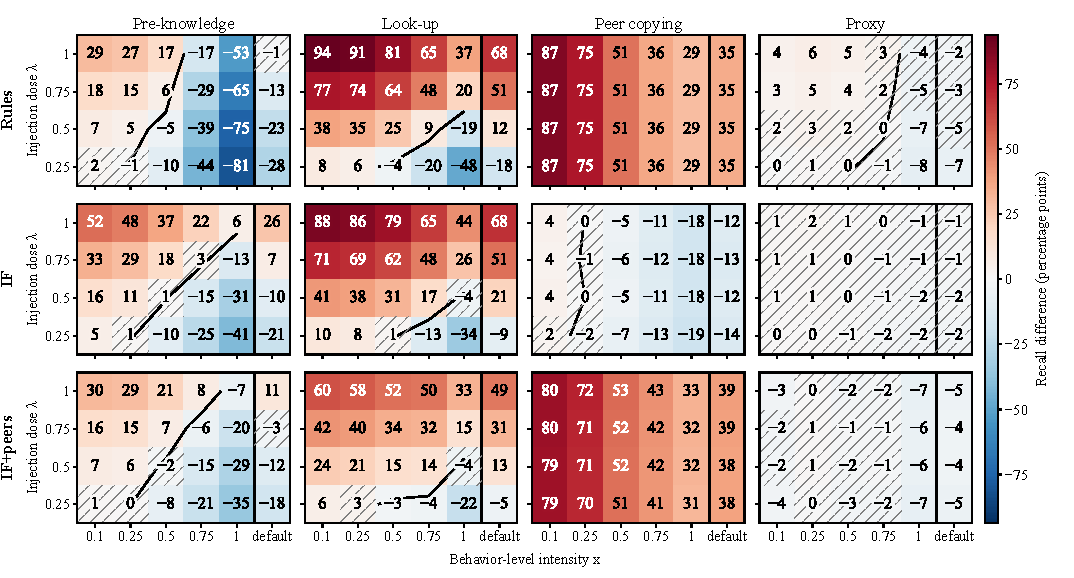
\includegraphics[width=0.90\textwidth]{fig_dose.pdf}
\caption{Recall difference between feature-aligned injection at dose $\lambda$ and behavior-level cheating at intensity $x$, in percentage points, by detector (rows) and type (columns); 10 replicates. Column ``default'' is the main configuration, separated by the vertical line. Hatched cells have a 95\% interval that includes zero; the black curve marks zero difference where the sign change exceeds these intervals.}
\label{fig:dose}
\end{figure*}

Across 60 joint configurations of ten mechanism and four injection parameters, the difference is positive in 98--100\% of configurations for look-up (medians 40--59\pp{}) and in 92--93\% for peer copying with the peer-aware detectors (medians 40--41\pp{}). For pre-knowledge it is positive in 42\% of configurations for the rules, 72\% for IF and 63\% for IF+peers, and for proxy it stays within $\pm 13$\pp{}.

\subsection{Which Cheaters Are Detected}
Table~\ref{tab:sub} separates the sub-populations that the mechanisms create. Pairs that submit together are detected by the rules and by IF+peers almost as reliably as injected collusion; pairs that submit separately are detected at 36--40\%. For these detectors, performance on ``collusion'' measures mostly whether colluding students submit within the 5\,s window that the peer features require, a condition the injection always satisfies. Among students with pre-knowledge, the forests detect about 10\% of those who disguise their timing.
\begin{table}[t]
\caption{Recall (\%) on Behavior-Level Cheating by Sub-Population, for the Frozen Detectors and Two Classical Indices}
\label{tab:sub}
\centering
\footnotesize
\setlength{\tabcolsep}{3.5pt}
\begin{tabular}{@{}lrrrrr@{}}
\toprule
Sub-population & Rules & IF & IF+peers & AS & PF \\
\midrule
Pre-knowledge, fast answers & 41.0 & 51.7 & 38.6 & -- & 16.9 \\
Pre-knowledge, disguised timing & 28.4 & 9.3 & 10.8 & -- & 2.0 \\
Copying, pair submits together & 92.0 & 21.5 & 86.0 & 52.6 & 44.5 \\
Copying, pair submits separately & 39.8 & 22.1 & 36.1 & 47.9 & 43.2 \\
\midrule
Injected collusion, for reference & 100.0 & 11.0 & 100.0 & 99.9 & 6.2 \\
\bottomrule
\multicolumn{6}{@{}l}{AS: answer similarity on incorrect answers. PF: response-time person-fit.}
\end{tabular}
\end{table}

\subsection{Robustness to the Protocol and to Honest Behavior}
Under variants of the protocol and of honest behavior (full table with the code), the overall difference stays between 20 and 36\pp{} for every detector under a threshold set without labels, an exam-like revision rate (0.84 changes per attempt, as observed in \cite{ranger2020eexams}), item sets drawn per attempt, and a fixed closing time at which unfinished attempts are submitted automatically. The variants are not neutral for single types: with item sets drawn per attempt the rules' recall on behavior-level copying falls from 65.5\% to 25.4\%. Purging matters more for the overall result. When the cheaters of the training cohorts (12\% of training attempts) are not removed before fitting, the forests lose 4--10\pp{} of recall, but the rules fall from 61.9\% to 26.1\% under injection and from 36.2\% to 20.6\% under behavior-level cheating, because the extreme and homogeneous injected values move the reference quantiles on which the rules depend. At the low prevalence (1.6\% of training attempts) the effect almost disappears: the rules' recall is 55.2\% and 28.5\%, and the difference between the worlds is 26.7\pp{}.

\subsection{Supervised and Classical Detectors}
A gradient-boosting classifier on the same fifteen features (Table~\ref{tab:sup}) loses 34.8\pp{} of recall when it is trained on injected labels and meets behavior-level cheating, and 69.9\pp{} on look-up; the inflation is not specific to unsupervised detection. Trained on behavior-level labels it detects 69.6\% of behavior-level cheating, 33.5\pp{} more than the best of the three frozen detectors. The features therefore carry the signal of these mechanisms; the unsupervised detectors do not find it, and a classifier trained on injected labels finds less than half of it for look-up.

\begin{table}[t]
\caption{Recall (\%) of a Supervised Classifier at the 5\% FPR Threshold of Its Training World}
\label{tab:sup}
\centering
\footnotesize
\begin{tabular}{@{}lrrrrr@{}}
\toprule
Trained $\rightarrow$ tested & All & Pre-kn. & Look-up & Copying & Proxy \\
\midrule
Injection $\rightarrow$ injection & 79.8 & 79.9 & 99.0 & 99.4 & 21.9 \\
Injection $\rightarrow$ behavior & 45.1 & 52.8 & 29.1 & 64.4 & 24.8 \\
Behavior $\rightarrow$ injection & 48.7 & 33.9 & 27.5 & 100.0 & 41.7 \\
Behavior $\rightarrow$ behavior & 69.6 & 77.2 & 75.6 & 75.2 & 34.5 \\
\bottomrule
\end{tabular}
\end{table}

The two classical indices are affected in the same way (Table~\ref{tab:sub}). An answer-similarity statistic detects 94.8\% of injected collusion and 47.0\% of behavior-level copying on all answers, and 99.9\% and 50.4\% when restricted to incorrect answers (the variant shown in the table). It is as inflated by the injection as the peer features are, but it does not depend on synchrony and exceeds IF+peers on pairs that submit separately. The response-time person-fit statistic detects 38.6\% of injected rapid responders and 9.4\% of behavior-level pre-knowledge. The local outlier factor \cite{breunig2000lof} and a one-class support vector machine \cite{scholkopf2001support} reproduce the pattern of Table~\ref{tab:main} for look-up and peer copying.

\subsection{Low Prevalence and Real Logs}
With cheating on 5\% of final attempts (realized FPR 3.2--4.2\%), the precision of the rules is 34.0\% on the original generator, 27.4\% under injection and 15.0\% under behavior-level cheating; for IF+peers the mean is 17--20\% in all three conditions, with a wide interval under behavior-level cheating (10.6--26.5\%).

Over 10 replicates, a classifier separates real EdNet attempts from attempts of the original generator almost perfectly (area under the curve 0.999) and from the calibrated simulator with 0.830 on timing, change and score features. Detectors without peer features (IF, and the rules restricted to the attempt-level features) that were fitted on the original generator flag 31.5\% and 39.1\% of real attempts at a nominal 5\%; fitted on the calibrated simulator they flag 11.4\% and 22.0\%. IF+peers flags 12.9\% and 5.3\%, but peer features are not meaningful in logs without a common timed quiz. When IF is refitted on real attempts it flags 4.9\% of them, but 12.6\% of the attempts in the fastest quartile of answer time. Part of the over-flagging may come from the change of format from a timed quiz to a self-paced tutor rather than from synthetic behavior.

\section{Discussion and Future Work}\label{sec:discussion}
At the constants that the platform's generator actually used, the same detectors on the same simulated students lose 23--26\pp{} of recall, between 42\% and 51\% of it, when feature-aligned injection is replaced by behavior-level cheating, mostly on look-up and, for the detectors with peer features, on peer copying. This is not a universal constant: the difference takes either sign as the doses change. The supportable claim is that recall measured on feature-aligned injection does not predict recall on behavior-level cheating.

Three properties of the recipes explain the result. \emph{Magnitude}: an injection can choose an effect size that no simulated behavior produces, such as 27 extra answer changes. \emph{Direction}: the recipes encode cheating as speed or as answer changes, whereas looking an answer up makes simulated students slower and more accurate, a footprint that no recipe produces. \emph{Co-design}: the collusion recipe always satisfies the synchrony condition under which the peer features are evaluated. Magnitude can be varied; direction and co-design cannot be repaired by tuning the dose.

The behavioral world is not ground truth either: a classifier still tells it from real logs, and its mechanisms rest on assumed parameters. Two observations limit how much this weakens the result. The gaps for look-up, and for peer copying with the peer-aware detectors, stay positive in 92--100\% of the sensitivity configurations, in which the shares of cheaters who disguise their timing, answer before correcting or submit together each range over 0--1. For pre-knowledge the behavioral world may be pessimistic: in the field experiment of Ranger \emph{et al.} \cite{ranger2020eexams}, response-time indicators detected about 40--60\% of students who had practiced eight of the 20 items at a 5\% false-positive rate. Here the detectors reach 15--18\% at a comparable coverage ($x = 0.5$) and 24--34\% at the default 0.65, although indicators and design differ. A higher behavioral recall would shrink the gap for that type only.

The same experiment qualifies our look-up mechanism. Students who received a note with all correct answers revised 6.58 answers on average, against 0.84 for regular examinees, which is closer to the injected ``excessive changes'' than to our look-up, although the injection adds about four times as many changes. A mechanism in which answers arrive late and are corrected in bulk was not simulated.

We recommend the following for evaluating log-based cheating detectors. (i) Do not define positive cases through the detector's own features or model family; if this is unavoidable, report the effect of the construction on every feature. (ii) Simulate cheating as behavior, vary the dose and the assumed parameters, and report sub-populations that the features single out, such as pairs that submit together. (iii) Freeze the detector before generating evaluation data, set thresholds without labels, and evaluate with and without purging of the training data. (iv) Set operating thresholds on real ordinary behavior of the target population and label synthetic results as synthetic.

\textbf{Limitations.} Both constructions are synthetic, and so is every detection result. The mechanism parameters are assumptions, and four mechanisms do not exhaust how students cheat. The recipes are those of one platform, the scoping sample was coded by a single author, and strict feature-aligned injection is uncommon in that sample, so the results show what happened with these recipes and why, not how large the problem is in the literature. The calibration data come from an ungraded tutor, not from examinations.

\textbf{Future work.} The simulated event stream will be replayed through the platform's quiz service to check that the deployed pipeline computes the same features. A consented pilot with real quiz logs is needed to test the detectors on verified cases, and experimental data with induced pre-knowledge \cite{toton2019preknowledge} would provide a labeled anchor for one mechanism.

\section{Conclusion}
When the anomalies used to evaluate a cheating detector are defined along the detector's own features, the evaluation says little about behavior that was not built that way. With detectors, students and cheaters held fixed, replacing the injection recipes of one platform by behavior-level cheating removed 23--26\pp{} of recall at a 5\% false-positive rate, most of it on look-up and, for the detectors with peer features, on peer copying. The same happened to a supervised classifier trained on injected labels, although the features carried enough signal for a classifier trained on behavior-level labels to find most cases. Detectors without peer features that were developed on synthetic ordinary behavior over-flagged real attempts two- to eightfold. Synthetic evaluation remains useful when cheating is modeled as behavior, its assumptions are varied, and its results are presented as what they are. The simulator, the calibration and all results are available at \url{https://github.com/Newterios/Examory}.

\section*{Acknowledgment}
The authors thank Y. Akhanov, who developed the anomaly-detection pipeline and the original data generator of the Examory platform that are evaluated in this work.
% To be completed by the corresponding author before submission: funding, if
% any, and the disclosure that the IEEE policy requires when AI-generated
% content (text, figures, code) is used in a paper.


\bibliographystyle{IEEEtran}
\bibliography{IEEEabrv,refs}

\end{document}
